% Options for packages loaded elsewhere
\PassOptionsToPackage{unicode}{hyperref}
\PassOptionsToPackage{hyphens}{url}
%
\documentclass[
  12pt,
  english,
  letterpaper,
  oneside,
  BCOR = 0 pt,
  singlespacing = true]{scrbook}
\title{\yourtitle}
\usepackage{etoolbox}
\makeatletter
\providecommand{\subtitle}[1]{% add subtitle to \maketitle
  \apptocmd{\@title}{\par {\large #1 \par}}{}{}
}
\makeatother
\subtitle{\yoursubtitle}
\author{\yourname}
\date{\yourdate}

\usepackage{amsmath,amssymb}
\usepackage{lmodern}
\usepackage{iftex}
\ifPDFTeX
  \usepackage[T1]{fontenc}
  \usepackage[utf8]{inputenc}
  \usepackage{textcomp} % provide euro and other symbols
\else % if luatex or xetex
  \usepackage{unicode-math}
  \defaultfontfeatures{Scale=MatchLowercase}
  \defaultfontfeatures[\rmfamily]{Ligatures=TeX,Scale=1}
  \setmainfont[Path=fonts/,Extension=.otf,UprightFont=*-regular,BoldFont=*-bold,ItalicFont=*-italic,BoldItalicFont=*-BoldItalic]{texgyretermes}
\fi
% Use upquote if available, for straight quotes in verbatim environments
\IfFileExists{upquote.sty}{\usepackage{upquote}}{}
\IfFileExists{microtype.sty}{% use microtype if available
  \usepackage[]{microtype}
  \UseMicrotypeSet[protrusion]{basicmath} % disable protrusion for tt fonts
}{}
\makeatletter
\@ifundefined{KOMAClassName}{% if non-KOMA class
  \IfFileExists{parskip.sty}{%
    \usepackage{parskip}
  }{% else
    \setlength{\parindent}{0pt}
    \setlength{\parskip}{6pt plus 2pt minus 1pt}}
}{% if KOMA class
  \KOMAoptions{parskip=half}}
\makeatother
\usepackage{xcolor}
\IfFileExists{xurl.sty}{\usepackage{xurl}}{} % add URL line breaks if available
\IfFileExists{bookmark.sty}{\usepackage{bookmark}}{\usepackage{hyperref}}
\hypersetup{
  pdflang={en},
  hidelinks,
  pdfcreator={LaTeX via pandoc}}
\urlstyle{same} % disable monospaced font for URLs
\usepackage[top=1in, left=1.5in, right=1in, bottom=1in, truedimen,
twoside=false, bindingoffset=0pt, nohead]{geometry}
\usepackage{listings}
\newcommand{\passthrough}[1]{#1}
\lstset{defaultdialect=[5.3]Lua}
\lstset{defaultdialect=[x86masm]Assembler}
\usepackage{longtable,booktabs,array}
\usepackage{calc} % for calculating minipage widths
% Correct order of tables after \paragraph or \subparagraph
\usepackage{etoolbox}
\makeatletter
\patchcmd\longtable{\par}{\if@noskipsec\mbox{}\fi\par}{}{}
\makeatother
% Allow footnotes in longtable head/foot
\IfFileExists{footnotehyper.sty}{\usepackage{footnotehyper}}{\usepackage{footnote}}
\makesavenoteenv{longtable}
\usepackage{graphicx}
\makeatletter
\def\maxwidth{\ifdim\Gin@nat@width>\linewidth\linewidth\else\Gin@nat@width\fi}
\def\maxheight{\ifdim\Gin@nat@height>\textheight\textheight\else\Gin@nat@height\fi}
\makeatother
% Scale images if necessary, so that they will not overflow the page
% margins by default, and it is still possible to overwrite the defaults
% using explicit options in \includegraphics[width, height, ...]{}
\setkeys{Gin}{width=\maxwidth,height=\maxheight,keepaspectratio}
% Set default figure placement to htbp
\makeatletter
\def\fps@figure{htbp}
\makeatother
\setlength{\emergencystretch}{3em} % prevent overfull lines
\providecommand{\tightlist}{%
  \setlength{\itemsep}{0pt}\setlength{\parskip}{0pt}}
\setcounter{secnumdepth}{5}
% The following package and toggle
% are needed to implement the switch
% between the PhD and MS templates.
% For now, it is used only on the title
% page.
\usepackage{etoolbox}
\newtoggle{ms}
%%%%%%%%%%%%%%%%%%
%%% To be filled %
%%%%%%%%%%%%%%%%%%

\newcommand{\yourtitle}{Dissertation Title, that can span    %
                        over multiple lines if needed}       % The title of your thesis
\newcommand{\yourname}{First Last}                           % Your name
\newcommand{\youradvisor}{Dr.\ Advisor}                      % The name of your advisor(s).
% The ".\ " makes sure the spacing after the dot is correct, cf. https://tex.stackexchange.com/a/2230/.
\newcommand{\yourkeywords}{Key1, Key2, A longer keyword}     % Separate your keywords with ",".
% One of the following two lines should be commented, and one should be un-commented.
%\togglefalse{ms}                                            % Comment this toggle if you are a PhD student.
\toggletrue{ms}                                              % Comment this toggle if you are a MS student
\newcommand{\yourdate}{2022-01-31}                           % Enter the date in the YYYY-MM-DD format. Only the month and year will be displayed on the cover 

%%%%%%%%%%%%%%%%%%%%%%%%%
%%%% Optional arguments %
%%%%%%%%%%%%%%%%%%%%%%%%%

% Adding a precise licence will make your work
% easier to share, cite and adapt.
% You can use
% https://guides.augusta.edu/c.php?g=796891&p=6003854
% or 
% https://www.aje.com/arc/creative-commons-intro/
% to help you decide on a licence.
\newcommand{\yourlicence}{\href{https://creativecommons.org/licenses/by/4.0/}{CC Attribution 4.0 International}}    % More precise licence.
% To pick a licence, you can use e.g. https://beza1e1.tuxen.de/licences/ or https://choosealicense.com/ to help you decide.

% \newcommand{\yoursubtitle}{Subtitle (Optional)}                                                                     % The subtitle.

% You can add a "mention", typically to 
% indicate that your manuscript is a draft
\newcommand{\yourmention}{Draft} 

%%%%%%%%%%%%%%%%%%%%%%%%
% ⚠ Do not edit ⚠      %
% what is below at all %
%%%%%%%%%%%%%%%%%%%%%%%%


%%%%%%%%%%%%
% Packages %
%%%%%%%%%%%%

\usepackage{scrhack}                               % Hack from the koma-script for various packages to play more nicely with this class.
\usepackage{xstring}                               % Used to perform substitution, using \StrSubstitut.
\usepackage[figure, table, lstlisting]{totalcount} % To conditionally insert list of figures, tables, and listings.
% https://tex.stackexchange.com/a/297657
% https://tex.stackexchange.com/a/297655
\usepackage[english]{datetime2}                    % To extract the month and year from the date.
\usepackage{chngcntr}                              % To obtain a "global numbering" of tables and figures.

%%%%%%%%%%%%%%
% Cover page %
%%%%%%%%%%%%%%


% We add some space after the subtitle if it
% is defined, after the title if not.
\ifdefined\yoursubtitle
    \makeatletter
        \apptocmd{\@subtitle}{\par}{}{}
    \makeatother
    \else
    \let\yoursubtitle\par\vspace{1em}
\fi

% We add "By", followed by a new line,
% before your name, and change the font 
% to 16pts.
\makeatletter
    \pretocmd{\@author}{By \\}{}{}
\makeatother

% The following extract the month and year
% from the date, and display them in the title.
\DTMsavedate{mydate}{\yourdate}
\makeatletter
    \renewcommand{\yourdate}{%
        \DTMenglishmonthname{\@dtm@month}\\
        \@dtm@year
    }
\makeatother

% This add some information between 
% your name and the date.
\makeatletter
    \pretocmd{\yourdate}{%
        \vspace{1em}
        Submitted to the Faculty of the Graduate School\\
        of Augusta University in partial fulfillment\\
        of the Requirements of the Degree of\\
        \iftoggle{ms}{Master of Science}{Doctor of Philosophy} % This toggle will display either 
                                                               % "Master of Science" or "Doctor of Philosophy"
                                                               % based on the choice made in info.tex.
        \vspace{1em}\par
    }{}{}
\makeatother

% This add copyright information, 
% abusing the "publisher" field.
\makeatletter
    \publishers{%
        \textcopyright~\@dtm@year{} \yourname%
        \ifdefined\yourlicence{\\[.1em] \yourlicence}
        \else
        \relax
        \fi
        \pagenumbering{gobble} % No page number on next page.
    }
\makeatother

%%%%%%%%%%%
% Margins %
%%%%%%%%%%%

% We do not want to add any additional margin space
% on the cover page
\renewcommand*{\coverpagetopmargin}{2in}
\renewcommand*{\coverpageleftmargin}{1.5in}
\renewcommand*{\coverpagerightmargin}{1in}
\renewcommand*{\coverpagebottommargin}{1in}

% We set all the margins to 0.
% Sorry about that, I know it is not pretty,
% but that is the only way I could content
% TGS's requirements on the template.
\setlength{\topmargin}{0pt}
\setlength{\headheight}{0pt}
\setlength{\headsep}{0pt}
\setlength{\columnsep}{0pt}
\setlength{\marginparsep}{0pt}
\setlength{\marginparpush}{0pt}
\setlength{\marginparwidth}{0pt}

% No space above chapters.
% https://tex.stackexchange.com/a/231940
\RedeclareSectionCommand[
  beforeskip=0pt
]{chapter}

%%%%%%%%%%%%%%%%%%%%%%%
% Headers and footers %
%%%%%%%%%%%%%%%%%%%%%%%

% We only want page numbers, no headers.
\pagestyle{plain}
% No page number for the first part of the document.
\thispagestyle{empty}


%%%%%%%%%%
% Titles %
%%%%%%%%%%

% Chapter titles should be centered.
\renewcommand\raggedchapter{\centering}

%%%%%%%%%%%%%
% Meta-data %
%%%%%%%%%%%%%

\hypersetup{
    pdftitle={\yourtitle},
    pdfauthor={\yourname},
    pdflang={en},
    pdfkeywords={\yourkeywords},
    pdfauthor={\yourname}
}


%%%%%%%%%
% Fonts %
%%%%%%%%%

% Some of the fonts parameters are set-up in the info.md file.
% The title is in small caps.
\setkomafont{title}{\scshape\Large}
% Figures and legends should be 10-point font. 
\addtokomafont{caption}{\small}
\addtokomafont{captionlabel}{\small}
% Subtitle and title should use the same font size.
\setkomafont{subtitle}{\scshape\Large}
% Author name should be 16 pts
\addtokomafont{author}{\Large}
% Date should be in smaller font.
\setkomafont{date}{\large}


%%%%%%%%%%%
% Spacing %
%%%%%%%%%%%


% Everything must be double spaced
\linespread{2}
% *but* the sectioning commands
% (titles, subtitles, etc.).
% https://tex.stackexchange.com/a/365269/
\addtokomafont{disposition}{\linespread{1}}
% Since biblatex is loaded quite late in the template 
% (cf. https://github.com/jgm/pandoc-templates/blob/master/default.latex )
% we defer this command, that let the line space in the references be only 
% single-spaced, to the end of the preamble.
\AtEndPreamble{
    \AtNextBibliography{\linespread{1}}
}


%%%%%%%%%%%%%%%%%%%%%%%%%%%%%%%%%%%%%%%
% Dedication, a.k.a. Acknowledgements % 
%%%%%%%%%%%%%%%%%%%%%%%%%%%%%%%%%%%%%%%

\pretocmd{\dedication}{%
    \chapter*{Acknowledgements}
    \pagenumbering{gobble}      % No page number
    \par                        % New paragraph
    {
        #1                      % Actual text
    }
    \clearpage                  % New page
}{}{}


%%%%%%%%%%%%
% Abstract % 
%%%%%%%%%%%%


% https://tex.stackexchange.com/a/40547
% https://tex.stackexchange.com/a/68227
\makeatletter
    \newenvironment{abstract}{%
        % At the beginning of the environment:
        \pagenumbering{gobble} % No page number.
        \chapter*{Abstract}
        {                       % This group must be single-spaced.
            \linespread{1}
            \textsc{\yourname} \\
            \@title \\
            Under the direction of \textsc{\youradvisor}
        }
        \\[3em]
      }%
     {%
      %  At the end of the environment:
      \\[3em] \textsc{Keywords}: \StrSubstitute{\yourkeywords}{,}{\textperiodcentered} % We list the keywords.
      \clearpage
      \pagestyle{empty}
      % The table of content
      % follows immediately (and automatically)
      % the abstract.
      \renewcaptionname{english}%
        {\contentsname}%
        {Table of Contents}  % We rename the table of contents.
      \tableofcontents        % Table of contents.
      \iftotaltables          % If there are tables in the document…
        \listoftables         % …write out the List of Tables
      \fi
      \iftotalfigures         % If there are figures in the document…
        \listoffigures        % …write out the List of Figures
      \fi
      \iftotallstlistings     % If there are listings in the document…
        \lstlistoflistings    % …write out the List of Listings.
      \fi
}
\makeatother

%%%%%%%%%%%%%%%%%%%%%%%%%%%%%%%%
% Names of tables and captions %
%%%%%%%%%%%%%%%%%%%%%%%%%%%%%%%%

% Since biblatex is loaded quite late in the template 
% (cf. https://github.com/jgm/pandoc-templates/blob/master/default.latex )
% we defer those commands, that let the references being in the table of contents.
% and make sure that the bibliography is treated as a chapter, and not a section.
\AtEndPreamble{
    \DeclarePrintbibliographyDefaults{heading=bibintoc} % We add the references in the table of contents
    \defbibheading{bibliography}[\bibname]{%
    \chapter*{#1}%
    \markboth{#1}{#1}}
}
% https://tex.stackexchange.com/a/544718
% We rename the simple "Listings" to "List of Listings"
\renewcommand{\lstlistlistingname}{List of Listings}
% https://stackoverflow.com/a/2709986

% Counters for figures, tables and listings
% are global, and not per chapter.
% https://tex.stackexchange.com/q/371184
\counterwithout{figure}{chapter}
\counterwithout{table}{chapter}
\lstset{numberbychapter=false}
% https://tex.stackexchange.com/a/595356

%%%%%%%%%%%%%%%%%%%%%%%%%%%%%%
% Mention (draft annotation) %
%%%%%%%%%%%%%%%%%%%%%%%%%%%%%%

\ifdefined\yourmention
\usepackage{draftwatermark}
\SetWatermarkText{\yourmention}
\SetWatermarkScale{2.27}
\SetWatermarkColor{augustagrey!20}
\fi
%%%%%%%%%%%%%%%%%%%%%%%%%%%%%%%%%%%%%%%%%%%%%%%%%%%
% Everything below can be freely edited.          % 
% Beware that it may break the compilation of     %
% the main demo file, though.                     %
%%%%%%%%%%%%%%%%%%%%%%%%%%%%%%%%%%%%%%%%%%%%%%%%%%%


%%%%%%%%%%%%%%%%%%%%%%
% Debugging packages %
%%%%%%%%%%%%%%%%%%%%%%

% \usepackage{showframe} % show the page layout
\usepackage{layouts}   
% Allow to use 
% \printinunitsof{in}{\pagevalues}
% to "see" the margins.

% The following commands allows to "see" the font sizes.
% cf. https://tex.stackexchange.com/a/24600
% https://texfaq.org/FAQ-csname
\makeatletter
\newcommand\thefontsize[1]{\csname #1\endcsname #1 is equivalent to \f@size pt\par}
\makeatother

\newcommand{\getfontsize}{
    \thefontsize{tiny}
    \thefontsize{scriptsize}
    \thefontsize{footnotesize}
    \thefontsize{small}
    \thefontsize{normalsize}
    \thefontsize{large}
    \thefontsize{Large}
    \thefontsize{LARGE}
    \thefontsize{huge}
    \thefontsize{Huge}
    \normalsize
}

%%%%%
% Emoji support for latex
%%%%%

\usepackage[verbose]{newunicodechar}

% List of symbols supported by Symbola at
% https://www.fileformat.info/info/unicode/font/symbola/list.htm

\newfontfamily\sym{Symbola}
\DeclareTextFontCommand{\symb}{\sym}

% The following unicode symbols are rendered in the 
% symbola font, as they do not exist in the main
% font of the template:
\newunicodechar{🔒}{\symb 🔒} % U+1F512, "LOCK"
\newunicodechar{✘}{\symb ✘} % U+2718,  "HEAVY BALLOT X"
\newunicodechar{⚠}{\symb ⚠} % U+26A0,  "WARNING SIGN"
\newunicodechar{❓}{\symb ❓} % U+2753, "BLACK QUESTION MARK ORNAMENT"
\newunicodechar{🔜}{\symb 🔜} % U+1F51C, "SOON WITH RIGHTWARDS ARROW ABOVE"
\newunicodechar{ℕ}{\symb ℕ} % U+2115,  "DOUBLE-STRUCK CAPITAL N"
\newunicodechar{ℤ}{\symb ℤ} % U+2124,  "DOUBLE-STRUCK CAPITAL Z"
\newunicodechar{✔}{\symb ✔} % U+2714,  "HEAVY CHECK MARK"
% More symbols for new lines: https://stackoverflow.com/a/18931703
\newunicodechar{↵}{\symb ↵} % U+21B5,  "DOWNWARDS ARROW WITH CORNER LEFTWARDS"
\newunicodechar{↲}{\symb ↲} % U+21B2,  "DOWNWARDS ARROW WITH TIP LEFTWARDS"
\newunicodechar{🛡}{\symb 🛡} % U+1F6E1, "SHIELD"
\newunicodechar{ℝ}{\symb ℝ} % U+211D,  "Double-Struck Capital R"
\newunicodechar{□}{\symb □} % U+25A1,  "White square"

% Note that you can also define unicode characters
% to be interpreted as latex commands, following
% https://tex.stackexchange.com/a/522961 :

\newunicodechar{↔}{\ensuremath{\leftrightarrow}}

%%%%%%%%%%%%%%%%%%%%%%%%%%%%%%%%%%%% 
% Colors                           %
% https://brand.augusta.edu/color/ %
%%%%%%%%%%%%%%%%%%%%%%%%%%%%%%%%%%%%

\usepackage{xcolor}
% Those are the "official" AU color, but we are assuming black-and-white printing.
\definecolor{augustablue}{HTML}{002f55} % Used for "external" links.
\definecolor{augustagrey}{HTML}{A5ACAF} % Used for "internal" links.

% Non-colored links, with underline, cf. https://tex.stackexchange.com/a/26085
% This allow the links to be visually present only if the document is viewed on a screen.
% Colored distribution inspired by https://tex.stackexchange.com/a/526148

% This is to add color to the footnotes.
\makeatletter
\def\@footnotecolor{red}
\define@key{Hyp}{footnotecolor}{%
 \HyColor@HyperrefColor{#1}\@footnotecolor%
}
\patchcmd{\@footnotemark}{\hyper@linkstart{link}}{\hyper@linkstart{footnote}}{}{}
\makeatother

% Setup new colors
\hypersetup{
    linkcolor=augustagrey,
    citecolor=augustagrey,
    filecolor=augustablue,
    urlcolor=augustablue,
    menucolor=augustagrey,
    runcolor=augustablue,
    linkbordercolor=augustagrey,
    citebordercolor=augustagrey,
    filebordercolor=augustablue,
    urlbordercolor=augustablue,
    menubordercolor=augustagrey,
    runbordercolor=augustablue,
    footnotecolor=augustagrey,
}

\makeatletter
\Hy@AtBeginDocument{%
  \def\@pdfborder{0 0 0}         % Overrides border definition set with colorlinks=true
  \def\@pdfborderstyle{/S/U/W 1} % Overrides border style set with colorlinks=true
                                 % Hyperlink border style will be underline of width 1pt
}
\makeatother


% For sideways figures and landscape pages.
\usepackage{pdflscape}

% For proper quotations.
\usepackage{csquotes}

% For math. environments
\usepackage{mathtools}
\usepackage{amsthm}

% For the BibTex logo, courtesy of https://tex.stackexchange.com/a/198472
\def\BibTeX{\textrm{B\kern-.05em\textsc{i\kern-.025em b}\kern-.08em T\kern-.1667em\lower.7ex\hbox{E}\kern-.125emX}}

\newtheorem{theorem}{Theorem}

%%%%%%%%%%%%%%%%%%%%%
% Code Presentation %
%%%%%%%%%%%%%%%%%%%%%

% We make listings be a bit more pretty,
% cf. https://tex.stackexchange.com/a/272133

\lstset{
    % Space skipped before code block    
    % Default style fors listings
    basicstyle=\small\ttfamily\linespread{4},
    % flexible columns
    columns=[l]flexible,
    commentstyle=\color[rgb]{0.127,0.427,0.514}\ttfamily\itshape,
    escapechar=@,
    % Enables ASCII chars 128 to 255
    extendedchars=true,
    % Frame only at the top and bottom
    frame=tb,
    % Coloring schemes
    identifierstyle=\color{black},
    keywordstyle=\color[HTML]{228B22}\bfseries,
    ndkeywordstyle=\color[HTML]{228B22}\bfseries,
    % Style for strings
    stringstyle=\ttfamily,
    % Style for comments
    commentstyle={\ttfamily\color[HTML]{228B22}},
    % Line numbers at the left, and tiny
    numbers=left,
    numberstyle=\tiny,
    % Automatic breaking of long lines
    breaklines=true,
    % Add the "↲" symbol whenever a line is broken.
    % The "↲" symbol is declared as a unicode symbol
    % in the other header file (head_a.tex).
    prebreak=\raisebox{0ex}[0ex][0ex]{↲},
    % How strings are formatted, and style of quote sign.
    stringstyle=\color[rgb]{0.639,0.082,0.082}\ttfamily,
    upquote=true,
    % Anything betweeen $ does not become LaTeX math mode
    mathescape=false,
    % Spaces are not displayed as a special character
    showstringspaces=false,
    % Size of tabulations
    tabsize=3,
    % Case sensitivity
    sensitive=true,
    % Position of captions is bottom
    captionpos=b,
    % We reduce the space between the caption and the code.
    % This seems to come from a strange interaction between 
    % the listings and caption packages,
    % cf. https://tex.stackexchange.com/a/365260/
    abovecaptionskip=-30pt,
    % Floating option
    float=H,
    % We increment the space before and after the listings.
    aboveskip=2em,
    belowskip=2em, 
}

\lstset{literate=%
   *{0}{{{\color{darkgray}0}}}1
    {1}{{{\color{darkgray}1}}}1
    {2}{{{\color{darkgray}2}}}1
    {3}{{{\color{darkgray}3}}}1
    {4}{{{\color{darkgray}4}}}1
    {5}{{{\color{darkgray}5}}}1
    {6}{{{\color{darkgray}6}}}1
    {7}{{{\color{darkgray}7}}}1
    {8}{{{\color{darkgray}8}}}1
    {9}{{{\color{darkgray}9}}}1
} 

% We define a style for the Coq programming language
% https://tex.stackexchange.com/a/620012/
% lstlisting coq style (inspired from a file of Assia Mahboubi)

\definecolor{dkgreen}{rgb}{0,0.6,0}
\definecolor{ltblue}{rgb}{0,0.4,0.4}
\definecolor{dkviolet}{rgb}{0.3,0,0.5}

\lstdefinelanguage{coq}{ 
    % Comments may or not include Latex commands
    texcl=false, 
    % Vernacular commands
    morekeywords=[1]{Section, Module, End, Require, Import, Export,
        Variable, Variables, Parameter, Parameters, Axiom, Hypothesis,
        Hypotheses, Notation, Local, Tactic, Reserved, Scope, Open, Close,
        Bind, Delimit, Definition, Let, Ltac, Fixpoint, CoFixpoint, Add,
        Morphism, Relation, Implicit, Arguments, Unset, Contextual,
        Strict, Prenex, Implicits, Inductive, CoInductive, Record,
        Structure, Canonical, Coercion, Context, Class, Global, Instance,
        Program, Infix, Theorem, Lemma, Corollary, Proposition, Fact,
        Remark, Example, Proof, Goal, Save, Qed, Defined, Hint, Resolve,
        Rewrite, View, Search, Show, Print, Printing, All, Eval, Check,
        Projections, inside, outside, Def},
    % Gallina
    morekeywords=[2]{forall, exists, exists2, fun, fix, cofix, struct,
        match, with, end, as, in, return, let, if, is, then, else, for, of,
        nosimpl, when},
    % Sorts
    morekeywords=[3]{Type, Prop, Set, true, false, option},
    % Various tactics, some are std Coq subsumed by ssr, for the manual purpose
    morekeywords=[4]{pose, set, move, case, elim, apply, clear, hnf,
        intro, intros, generalize, rename, pattern, after, destruct,
        induction, using, refine, inversion, injection, rewrite, congr,
        unlock, compute, ring, field, fourier, replace, fold, unfold,
        change, cutrewrite, simpl, have, suff, wlog, suffices, without,
        loss, nat_norm, assert, cut, trivial, revert, bool_congr, nat_congr,
        symmetry, transitivity, auto, split, left, right, autorewrite},
    % Terminators
    morekeywords=[5]{by, done, exact, reflexivity, tauto, romega, omega,
        assumption, solve, contradiction, discriminate},
    % Control
    morekeywords=[6]{do, last, first, try, idtac, repeat},
    % Comments delimiters, we do turn this off for the manual
    morecomment=[s]{(*}{*)},
    % String delimiters
    morestring=[b]",
    morestring=[d],
    % Style for (listings') identifiers
    identifierstyle={\ttfamily\color{black}},
    % Style for declaration keywords
    keywordstyle=[1]{\ttfamily\color{dkviolet}},
    % Style for gallina keywords
    keywordstyle=[2]{\ttfamily\color{dkgreen}},
    % Style for sorts keywords
    keywordstyle=[3]{\ttfamily\color{ltblue}},
    % Style for tactics keywords
    keywordstyle=[4]{\ttfamily\color{dkblue}},
    % Style for terminators keywords
    keywordstyle=[5]{\ttfamily\color{dkred}},
    %Style for iterators
    % keywordstyle=[6]{\ttfamily\color{dkpink}},
    literate=
    {\\forall}{{\color{dkgreen}{$\forall\;$}}}1
    {\\exists}{{$\exists\;$}}1
    {<-}{{$\leftarrow\;$}}1
    {=>}{{$\Rightarrow\;$}}1
    {==}{{\code{==}\;}}1
    {==>}{{\code{==>}\;}}1
    %    {:>}{{\code{:>}\;}}1
    {->}{{$\rightarrow\;$}}1
    {<->}{{$\leftrightarrow\;$}}1
    {<==}{{$\leq\;$}}1
    {\#}{{$^\star$}}1 
    {\\o}{{$\circ\;$}}1 
    {\@}{{$\cdot$}}1 
    {\/\\}{{$\wedge\;$}}1
    {\\\/}{{$\vee\;$}}1
    {++}{{\code{++}}}1
    {~}{{\ }}1
    {\@\@}{{$@$}}1
    {\\mapsto}{{$\mapsto\;$}}1
    {\\hline}{{\rule{\linewidth}{0.5pt}}}1
    %
}[keywords,comments,strings]

%%%%%%%%%%%%%%%
% Derivations %
%%%%%%%%%%%%%%%

% We recommend using the more modern ebproof over
% the more "traditional" bussproofs,
\usepackage{ebproof}
\ifXeTeX
  % Load polyglossia as late as possible: uses bidi with RTL langages (e.g. Hebrew, Arabic)
  \usepackage{polyglossia}
  \setmainlanguage[]{english}
\else
  \usepackage[main=english]{babel}
% get rid of language-specific shorthands (see #6817):
\let\LanguageShortHands\languageshorthands
\def\languageshorthands#1{}
\fi
\ifLuaTeX
  \usepackage{selnolig}  % disable illegal ligatures
\fi
\usepackage[backend=biber]{biblatex}
\addbibresource{./references/references.bib}

\begin{document}
\frontmatter
\maketitle

\mainmatter
\dedication{
This part serves two purposes.\\[1em]
To write the acknowledgments (as a \enquote{\emph{Thank you note}}).
You can look for inspiration~\cite{Chisholm} if you need some.\\[1em]
To include a detailed summary of the work performed by other authors on published or accepted manuscripts used in the thesis / dissertation, if applicable.
}

\begin{abstract}
The abstract must not exceed 350 words.
It must consist of the briefest possible summary of the thesis / dissertation and the conclusions reached.
Explanatory matter and opinion must be omitted.
\end{abstract}

\cleardoublepage
\pagenumbering{arabic}

\hypertarget{introduction}{%
\chapter{Introduction}\label{introduction}}

This document is a guide on how to use it (``how meta!''), and its
structure does not reflect the structure of a Thesis: you will need to
erase (almost) all of its body and fill it with your own, organized in a
coherent manner respectful of your reader's expectations, of your fields
guidelines, and in agreement with your advisor.

It is very important that you comply with all of the graduate school's
policies \autocite{gradschool_policies}. This template was carefully
crafted with highest standards in mind, and respects all of the graduate
schools requirements. You can find additional information on the
\href{https://guides.augusta.edu/graduateschool/template}{``The Graduate
School Reference Center: ETD Templates \& Preparation Booklet''} or,
more generally, on
\href{https://github.com/aubertc/au_ccs_dissertation_template}{this
template's repository}.

Normally, what you can and cannot edit is clearly labeled in the source
code, either at the beginning of the file, or with

\begin{quote}
⚠ Do not edit ⚠
\end{quote}

\begin{description}
\tightlist
\item[Markdown only]
The comments applicable only to the markdown version of this document
are indicated in such environments.
\end{description}

\hypertarget{title-levels}{%
\section{Title Levels}\label{title-levels}}

As indicated in the koma-script manual, the class
\passthrough{\lstinline!scrbook!} that is used for this document has
access to 6 levels of titles:

\begin{lstlisting}
\chapter{Test}
\section{Test}
\subsection{Test}
\subsubsection{Test}
\paragraph{Test}
\subparagraph{Test}
\end{lstlisting}

Only Chapters, Sections and Subsections will appear in the table of
contents, by design.

\begin{description}
\tightlist
\item[Markdown only]
Note that pandoc's \passthrough{\lstinline!\#!} corresponds to Chapter,
and that increasing the number of \passthrough{\lstinline!\#!} increases
the level of heading.
\end{description}

\hypertarget{subsection}{%
\subsection{Subsection}\label{subsection}}

This is a subsection.

\hypertarget{subsubsection}{%
\subsubsection{Subsubsection}\label{subsubsection}}

This is a subsubsection.

\hypertarget{paragraph}{%
\paragraph{Paragraph}\label{paragraph}}

This is a paragraph.

\hypertarget{sub-paragraph}{%
\subparagraph{Sub-Paragraph}\label{sub-paragraph}}

This is a sub-paragraph.

\hypertarget{debugging}{%
\section{Debugging}\label{debugging}}

If this template does not ``work'' as expected, feel free to
\href{https://github.com/aubertc/au_ccs_dissertation_template/issues}{open
an issue} or reach out to
\href{https://spots.augusta.edu/caubert/\#contact}{the maintainer},
after having looked at \passthrough{\lstinline!aux/input.log!} as
(probably) indicated by latexmk.

\hypertarget{references-and-bibliography}{%
\chapter{References and
Bibliography}\label{references-and-bibliography}}

Prepare your references using \LaTeX's bibliography system
\href{http://www.bibtex.org/Using/}{\BibTeX}: this template uses by
default \href{https://pandoc.org/MANUAL.html\#citations}{biblatex}, but
you can \href{https://pandoc.org/MANUAL.html\#citation-rendering}{alter
this behaviour} to use \href{https://www.ctan.org/pkg/natbib}{natbib} if
you prefer.

The references are stored in the .bib file located at
\passthrough{\lstinline!references/references.bib!}: it contains
examples of various entries. In computer science, a good source of
bibliographical references is the \href{https://dblp.org/}{dblp computer
science bibliography}. Make sure to include the
\href{http://dx.doi.org/}{digital object identifier} (DOI) whenever
possible, and note that this identifier can
\href{https://www.doi2bib.org/}{be used to obtain the corresponding .bib
entry}. Finally, you can ``tidy'' your .bib file using
\href{https://flamingtempura.github.io/bibtex-tidy/}{bibtex-tidy}.

The list of references is automatically inserted in
\protect\hyperlink{chap:references}{the list of references},
p.~\pageref{chap:references}. Use \LaTeX's
\passthrough{\lstinline!\\cite!} command to insert references.

Links are only underlined \emph{on screen} (and not in print), and with
colors that should be
\href{https://tex.stackexchange.com/a/526148}{colourblind safe}.

\begin{description}
\item[Markdown only]
You can use various syntaxes to integrate references: on top of \LaTeX's
\passthrough{\lstinline!\\cite!} command,
\href{https://pandoc.org/MANUAL.html\#citation-syntax}{pandoc's}
\passthrough{\lstinline![@key]!}, as well as
\href{https://github.com/jgm/pandoc/issues/2335}{more complex commands},
such as \passthrough{\lstinline!\\citeauthor!} or pandoc's prefix,
locator, and suffix, such as in
\passthrough{\lstinline![see @key1, pp. 33-35 and *passim*; @key2, chap. 1]!}.

You can insert
\href{https://pandoc.org/MANUAL.html\#links-1}{hyperlinks} in different
ways, including hyperlinks to this document\footnote{You may note that
  the footnote number is itself a link.} using e.g.~the
\protect\hyperlink{introduction}{link automatically added to all
chapters}, following the convention described
\href{https://pandoc.org/MANUAL.html\#heading-identifiers}{in pandoc's
manual}.
\end{description}

\hypertarget{writing-mathematics}{%
\chapter{Writing Mathematics}\label{writing-mathematics}}

\LaTeX can be used to render
\href{https://en.m.wikibooks.org/wiki/LaTeX/Mathematics}{complex
mathematics expressions} in a relatively simple manner. Note that thanks
to XeLaTeX, you can insert mathematical symbols directly
\href{https://en.wikipedia.org/wiki/Mathematical_operators_and_symbols_in_Unicode}{in
unicode}, as follows: \(∀ y ∈ ℕ, ∃ x ∈ ℕ, y = x²\), but of course you
can always fall back to usual \LaTeX{} notation, using
e.g.~\passthrough{\lstinline!\\forall!} to produce \(\forall\).

You can add additional unicode symbols that may not be supported by this
template or its font using the model

\begin{lstlisting}
\newunicodechar{<unicode symbol>}{\ensuremath{<latex command>}}
\end{lstlisting}

(in \passthrough{\lstinline!head\_a.tex!} in the markdown version), in
this case additionally forcing the symbol
\passthrough{\lstinline!<unicode symbol>!} to be rendered in math mode
using \passthrough{\lstinline!\\ensuremath!}.

\hypertarget{theorem-proof-and-others-environments}{%
\section{Theorem, Proof, and Others
Environments}\label{theorem-proof-and-others-environments}}

\begin{description}
\item[Markdown only]
You can state e.g.~theorems and proofs using pandoc's built-in
\href{https://pandoc.org/MANUAL.html\#definition-lists}{``\emph{Definition
list}''}, that are rendered as \passthrough{\lstinline!description!}
environments in \LaTeX.

\begin{description}
\tightlist
\item[Theorem]
Every \(n ∈ ℕ\), \(n >1\) has a unique prime factorization.
\item[Proof]
Carl Friedrich Gauss told me so. \qed
\end{description}
\end{description}

To insert numbered theorems, definitions, and the like, and be able to
reference them or add automatically the ``qed'' (□) symbol, you need to
use \LaTeX's \passthrough{\lstinline!theorem!} environment,
\passthrough{\lstinline!label!} commands, etc.

\begin{theorem}[Pythagoras theorem]
\label{thm:pythagoras}
    \(∀ a, b, c, a²+b²=c²\).
\end{theorem}

\begin{proof}
    Proving \autoref{thm:pythagoras} is not that easy.
\end{proof}

\begin{description}
\tightlist
\item[Markdown only]
If you would rather keep the ``pure'' markdown syntax but improve pandoc
using a filter, you can look at
\href{https://github.com/jdutant/statement}{the pandoc filter
``statement''} and its
\href{https://github.com/jdutant/statement\#related-filters}{discussion
on related filters}, but it may be more difficult to install and use
properly.
\end{description}

\hypertarget{formal-proofs}{%
\section{Formal Proofs}\label{formal-proofs}}

You can easily represent formal proofs using \LaTeX's ebproof or
bussproof packages:

\begin{center}
    \begin{prooftree}
        \hypo{A \vee B}
        \hypo{[A]}
        \ellipsis{}{C }
        \hypo{[B] }
        \ellipsis{}{C }
        \infer3[$\vee\textrm{E}$]{C}
    \end{prooftree}
\end{center}

\hypertarget{figures-tables-code-listings-and-landscape-pages}{%
\chapter{Figures, Tables, (Code) Listings and Landscape
Pages}\label{figures-tables-code-listings-and-landscape-pages}}

\hypertarget{figures}{%
\section{Figures}\label{figures}}

\begin{description}
\tightlist
\item[Markdown only]
You can easily insert
\href{https://pandoc.org/MANUAL.html\#images}{images and figures} using
Pandoc, as in \autoref{fig:d_un_autre_age}, a painting by
\href{http://jeromeminard.com/travaux/}{Jérôme Minard} under
\href{https://forceg.jimdofree.com/licence-art-libre/}{copyleft}.
\end{description}

\begin{figure}
\centering
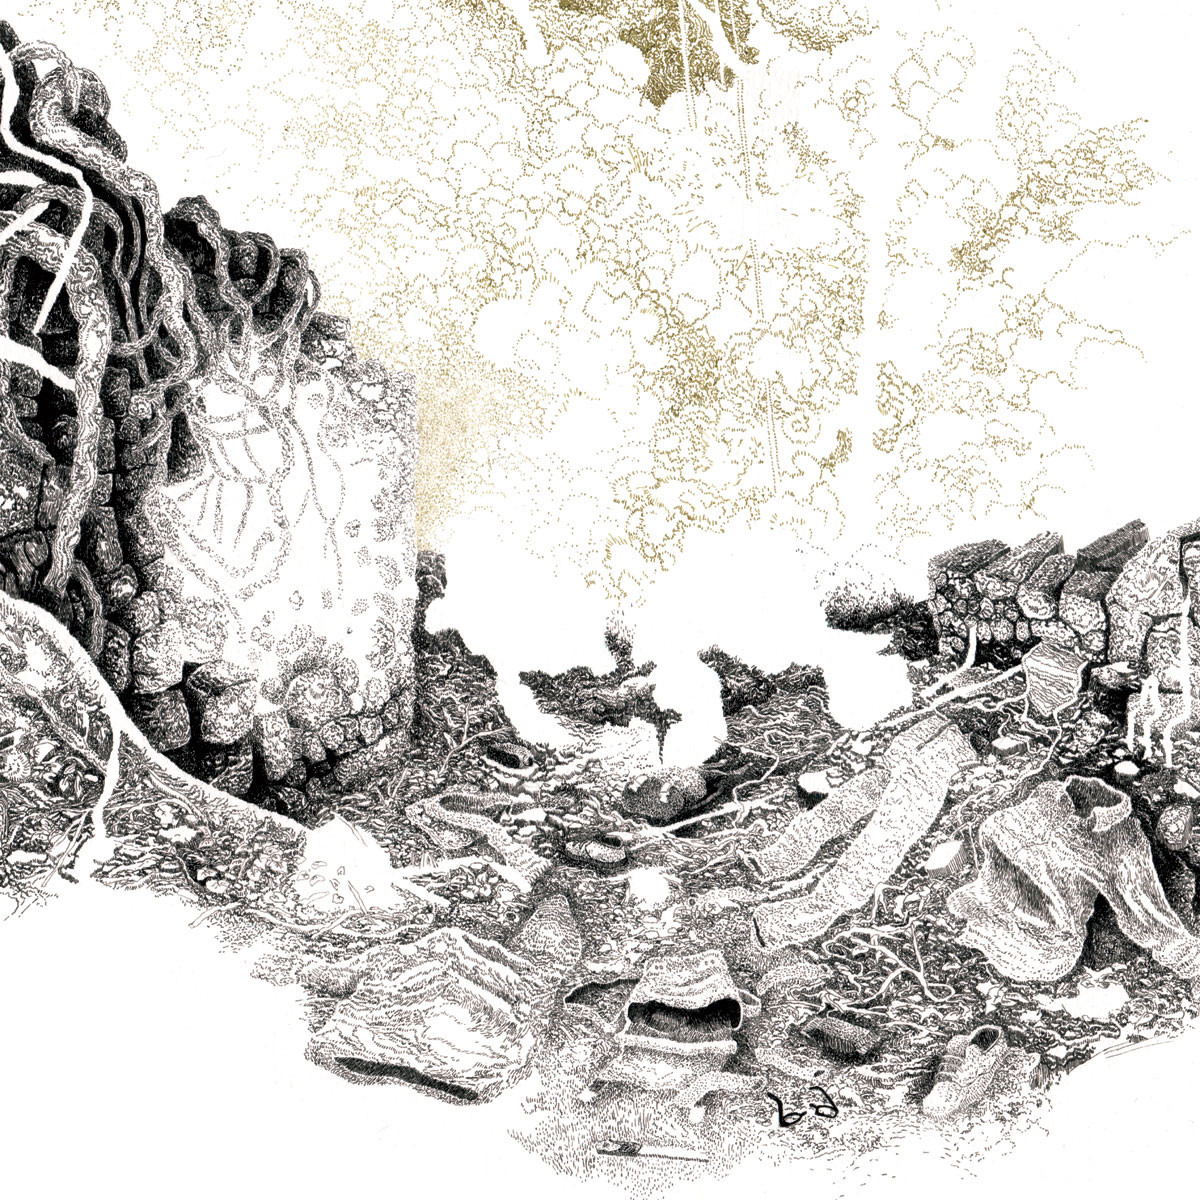
\includegraphics[width=0.8\textwidth,height=\textheight]{pictures/D_un_autre_age.jpg}
\caption{\emph{D'un autre âge}\label{fig:d_un_autre_age}}
\end{figure}

\hypertarget{tables}{%
\section{Tables}\label{tables}}

\begin{description}
\tightlist
\item[Markdown only]
You can write tables using
\href{https://pandoc.org/MANUAL.html\#tables}{pandoc's syntax\emph{es}},
as in Tables \ref{tbl:demo1}, \ref{tbl:demo2} and \ref{tbl:demo3} (all
borrowed from
\url{https://www.flutterbys.com.au/stats/tut/tut17.3.html}).
\end{description}

\begin{longtable}[]{@{}
  >{\raggedright\arraybackslash}p{(\columnwidth - 4\tabcolsep) * \real{0.15}}
  >{\centering\arraybackslash}p{(\columnwidth - 4\tabcolsep) * \real{0.17}}
  >{\raggedleft\arraybackslash}p{(\columnwidth - 4\tabcolsep) * \real{0.17}}@{}}
\caption{The price of categories \label{tbl:demo1}}\tabularnewline
\toprule
Column A & Column B & Column C \\
\midrule
\endfirsthead
\toprule
Column A & Column B & Column C \\
\midrule
\endhead
Category 1 High & High 95.00 & 100.00 \\
Category 2 High & High 82.50 & 80.50 \\
\bottomrule
\end{longtable}

\begin{longtable}[]{@{}llcr@{}}
\caption{Illustrating how to align entries in a table
\label{tbl:demo2}}\tabularnewline
\toprule
Default & Left & Center & Right \\
\midrule
\endfirsthead
\toprule
Default & Left & Center & Right \\
\midrule
\endhead
High & Cat 1 & A & 100.00 \\
High & Cat 2 & B & 85.50 \\
Low & Cat 3 & C & 80.00 \\
\bottomrule
\end{longtable}

\begin{longtable}[]{@{}
  >{\raggedright\arraybackslash}p{(\columnwidth - 4\tabcolsep) * \real{0.22}}
  >{\raggedright\arraybackslash}p{(\columnwidth - 4\tabcolsep) * \real{0.22}}
  >{\raggedright\arraybackslash}p{(\columnwidth - 4\tabcolsep) * \real{0.29}}@{}}
\caption{The price and advantages of fruits
\label{tbl:demo3}}\tabularnewline
\toprule
Fruit & Price & Advantages \\
\midrule
\endfirsthead
\toprule
Fruit & Price & Advantages \\
\midrule
\endhead
Bananas & \$1.34 & \begin{minipage}[t]{\linewidth}\raggedright
\begin{itemize}
\tightlist
\item
  built-in wrapper
\item
  bright color
\end{itemize}
\end{minipage} \\
Oranges & \$2.10 & \begin{minipage}[t]{\linewidth}\raggedright
\begin{itemize}
\tightlist
\item
  cures scurvy
\item
  tasty
\end{itemize}
\end{minipage} \\
\bottomrule
\end{longtable}

\hypertarget{code-listings}{%
\section{Code Listings}\label{code-listings}}

Code is displayed using the listings package. Check the ``Table 1:
Predefined languages'' of the listings package documentation to see the
list of supported languages by default.

\begin{description}
\tightlist
\item[Markdown only]
Your can display code using
\href{https://pandoc.org/MANUAL.html\#verbatim-code-blocks}{various
possible syntaxes}.
\end{description}

As a fenced block:

\begin{lstlisting}[language=Java]
public class HelloWorld {
    public static void main(String[] args) {
        System.out.println("Hello, World");
    }
}
\end{lstlisting}

In a figure, as in Listings \ref{lst:demo1}, \ref{lst:demo2} or
\ref{lst:demo3} (that uses respectively the backtick, the tildes, and
\passthrough{\lstinline!listinputlisting!} to display the code -- this
latter option allows to load a file directly).

\begin{lstlisting}[language=coq, caption={An inductive definition in Coq}, label={lst:demo1}]
(** Courtesy of https://coq.inria.fr/a-short-introduction-to-coq. **)
Inductive even : N -> Prop :=
| even_0 : even 0
| even_S n : odd n -> even (n + 1)
with odd : N -> Prop :=
| odd_S n : even n -> odd (n + 1).
\end{lstlisting}

\begin{lstlisting}[language=bash, caption={How to use braces (\{and \}) in bash}, label={lst:demo2}]
# Courtesy of https://stackoverflow.com/a/2188369
for num in {000..2}; do echo "$num"; done
\end{lstlisting}

\lstinputlisting[language=C, caption={"\emph{Hello World}" in C}, label={lst:demo3}]{code/hello_world.c}

\hypertarget{landscape-pages}{%
\section{Landscape Pages}\label{landscape-pages}}

You can obtain landscape pages using the landscape package in \LaTeX.

\begin{description}
\tightlist
\item[Markdown only]
This feature is not accessible in pure markdown: if you want to have
landscape pages, you need to use \LaTeX commands in your document.
\end{description}

Note that the drawing presented in \autoref{fig:language} was obtained
using \LaTeX's package tiKz, and that the source code is shared in the
pictures folder.

\begin{landscape}
    \vspace*{\fill} 
    \begin{figure}
        \centering
        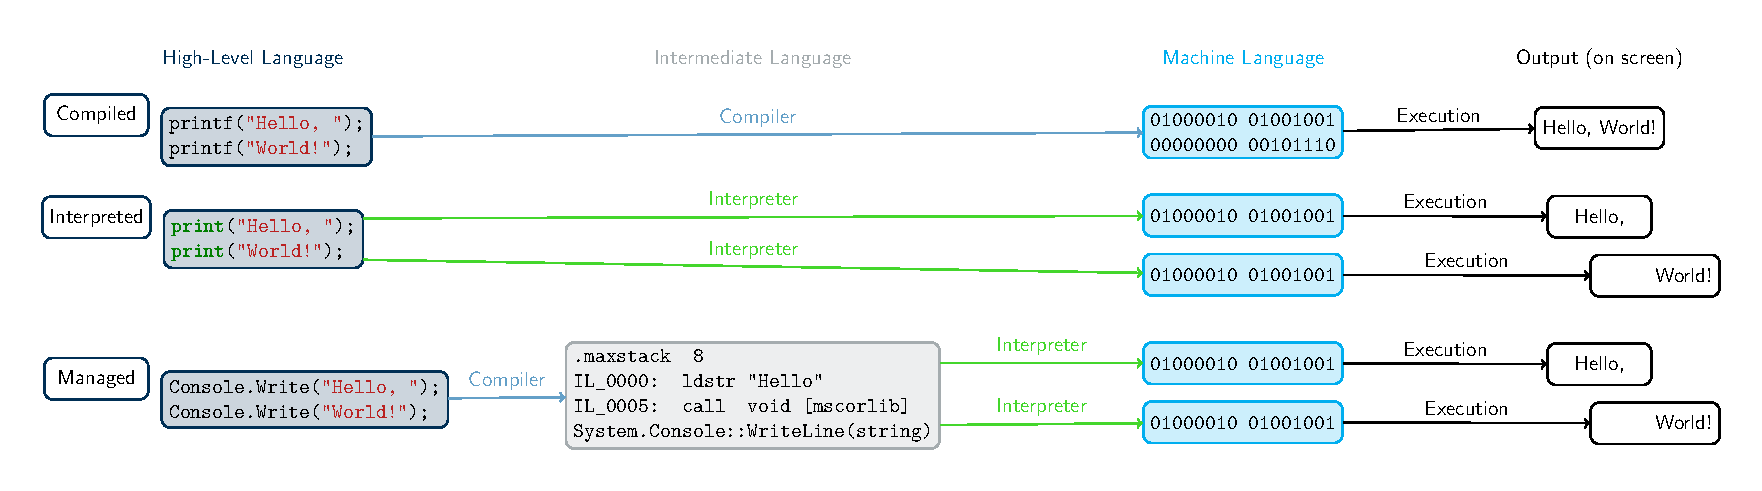
\includegraphics{pictures/languages_overview.pdf}
        \caption{Difference between programming languages (simplified)}
        \label{fig:language}
    \end{figure}
    \vspace*{\fill}
\end{landscape}

\hypertarget{margins-and-fonts}{%
\chapter{Margins and Fonts}\label{margins-and-fonts}}

\hypertarget{margins}{%
\section{Margins}\label{margins}}

The margin have been set to fit the graduate school's requirements to:

\begin{center}\rule{0.5\linewidth}{0.5pt}\end{center}

\printinunitsof{in}{\pagevalues}

\begin{center}\rule{0.5\linewidth}{0.5pt}\end{center}

Please, do not change those values.

\hypertarget{fonts}{%
\section{Fonts}\label{fonts}}

The font used is the font
\href{http://www.gust.org.pl/projects/e-foundry/tex-gyre/termes}{``TeX
Gyre Termes Font Family''}, which is an extension of the standard Times
New Roman that is free for commercial use, and can be
\href{https://www.gust.org.pl/fonts/licenses/GUST-FONT-LICENSE.txt}{freely
distributed}. It is set to 12pt in all of the document, and adjusted
when needed to the appropriate size (particularly in the page, where
most attributes need to be set at 16pts).

The ``usual'' correspondance between points and latex commands is as
follows:

\getfontsize

\clearpage
\printbibliography[label=chap:references, title=References]
\let\printbibliography\relax

\appendix

\hypertarget{appendix-a-optional}{%
\chapter{Appendix A (Optional)}\label{appendix-a-optional}}

Insert here protocols, figures not included, larger listings, etc.

\backmatter
\printbibliography

\end{document}
